\documentclass[11pt]{article}
\usepackage[margin=2cm]{geometry}

% Core packages
\usepackage{amsmath,amssymb}
\usepackage{tikz}
\usepackage{tikz-cd}
\usepackage{multicol}
\usepackage[backend=biber,style=authoryear]{biblatex}
\addbibresource{bibliography.bib}

% Paragraphs
\setlength{\parindent}{0pt}
\setlength{\parskip}{1\baselineskip}

\title{Taller 3\\[0.5em]
\large Astrofísica Moderna\\
Universidad de Antioquia}
\author{Daniel Soto Villada}
\date{\today}

\begin{document}
\maketitle

\begin{enumerate}
    \item Un electrón en la atmósfera de una enana blanca está confinado a una capa de espesor $\Delta x = 2.0 \times 10^{-10}\,\mathrm{m}$. Utilice el principio de incertidumbre para estimar la incertidumbre mínima en el momento $\Delta p$. Convierta $\Delta p$ en una energía cinética mínima $K_{\min}$ y compárela con $k_B T$ para $T = 1.0 \times 10^5\,\mathrm{K}$.

    \textit{Solución.} Usamos la relación de incertidumbre $\Delta x\,\Delta p\geq\hbar/2$. La incertidumbre mínima se obtiene al tomar la igualdad:
    \[
        \Delta p_{\min}=\frac{\hbar}{2\Delta x}
        =\frac{1.055\times10^{-34}\,\mathrm{J\,s}}
        {2(2.0\times10^{-10}\,\mathrm{m})}
        =2.64\times10^{-25}\,\mathrm{kg\,m\,s^{-1}}.
    \]
    Como $\Delta p_{\min}/m_e\simeq2.9\times10^5\,\mathrm{m\,s^{-1}}\ll c$, es consistente usar la expresión no relativista $K=(\Delta p)^2/(2m_e)$. Así,
    \[
        K_{\min}=3.82\times10^{-20}\,\mathrm{J}=0.238\,\mathrm{eV},
        \qquad k_BT=(1.381\times10^{-23})(1.0\times10^5)
        =1.38\times10^{-18}\,\mathrm{J}=8.62\,\mathrm{eV}.
    \]
    Por tanto, $K_{\min}/(k_BT)\simeq2.76\times10^{-2}$: la energía mínima asociada a la localización es aproximadamente el $2.8\%$ de la energía térmica $k_BT$. \parencite[Secs. 16.4, pp. 545--546; 18.5, p. 606]{chaparro2026}
    \begin{figure}[htbp]
    \centering
    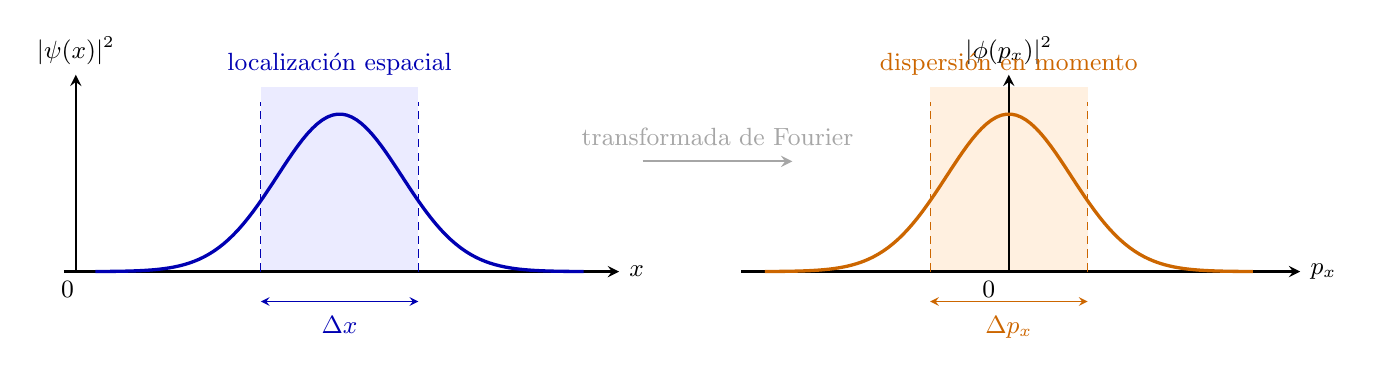
\begin{tikzpicture}[>=stealth, every node/.style={font=\small}]
        \fill[blue!8] (-1,0) rectangle (1,2.35);
        \draw[->,thick] (-3.5,0) -- (3.55,0) node[right] {$x$};
        \draw[->,thick] (-3.35,0) -- (-3.35,2.5) node[above] {$|\psi(x)|^2$};
        \draw[densely dashed,blue!70!black] (-1,0) -- (-1,2.15);
        \draw[densely dashed,blue!70!black] (1,0) -- (1,2.15);
        \draw[very thick,blue!70!black,domain=-3.1:3.1,samples=100]
            plot (\x,{2.0*exp(-0.8*\x*\x)});
        \draw[<->,blue!70!black] (-1,-0.38) -- (1,-0.38)
            node[midway,below=2pt] {$\Delta x$};
        \node[blue!70!black,above] at (0,2.37) {localización espacial};
        \node[below left] at (-3.25,0) {$0$};

        \fill[orange!12] (7.5,0) rectangle (9.5,2.35);
        \draw[->,thick] (5.1,0) -- (12.2,0) node[right] {$p_x$};
        \draw[->,thick] (8.5,0) -- (8.5,2.5) node[above] {$|\phi(p_x)|^2$};
        \draw[densely dashed,orange!80!black] (7.5,0) -- (7.5,2.15);
        \draw[densely dashed,orange!80!black] (9.5,0) -- (9.5,2.15);
        \draw[very thick,orange!80!black,domain=-3.1:3.1,samples=100]
            plot ({8.5+\x},{2.0*exp(-0.8*\x*\x)});
        \draw[<->,orange!80!black] (7.5,-0.38) -- (9.5,-0.38)
            node[midway,below=2pt] {$\Delta p_x$};
        \node[orange!80!black,above] at (8.5,2.37) {dispersión en momento};
        \node[below left] at (8.45,0) {$0$};

        \draw[->,gray!70,thick] (3.85,1.4) -- (5.75,1.4)
            node[midway,above=2pt] {transformada de Fourier};
    \end{tikzpicture}
    \caption{Esquema de la relación entre la localización de un paquete de onda y su distribución de momentos. Las curvas son ilustrativas; al reducir $\Delta x$ aumenta la dispersión $\Delta p_x$, de acuerdo con $\Delta x\,\Delta p_x\geq\hbar/2$.}
    \label{fig:incertidumbre}
\end{figure}

    \item Se observa una línea de una nebulosa planetaria en $486.1\,\mathrm{nm}$. Demuestre que la línea pertenece a la serie de Balmer e identifique los números cuánticos de la transición $n_i \to n_f$. Calcule la energía del fotón en eV. (Constante de Rydberg $R_\infty = 1.097 \times 10^7\,\mathrm{m}^{-1}$.)

    \textit{Solución.} Para las líneas del hidrógeno,
    \[
        \frac{1}{\lambda}=R_\infty\left(\frac{1}{n_f^2}-\frac{1}{n_i^2}\right),
        \qquad n_i>n_f.
    \]
    La serie de Balmer corresponde a $n_f=2$. Para la transición $4\to2$,
    \[
        \lambda_{4\to2}=\frac{1}{R_\infty(1/2^2-1/4^2)}
        =\frac{16}{3R_\infty}=486.2\,\mathrm{nm},
    \]
    en acuerdo con los $486.1\,\mathrm{nm}$ observados; por ello, $n_i=4$ y $n_f=2$ (línea H$\beta$). La energía del fotón es
    \[
        E_\gamma=\frac{hc}{\lambda}
        =\frac{(4.136\times10^{-15}\,\mathrm{eV\,s})(2.998\times10^8\,\mathrm{m\,s^{-1}})}
        {486.1\times10^{-9}\,\mathrm{m}}
        =2.55\,\mathrm{eV}.
    \]
    \parencite[Secs. 15.5--15.6, pp. 496, 503]{chaparro2026}
    \begin{figure}[htbp]
    \centering
    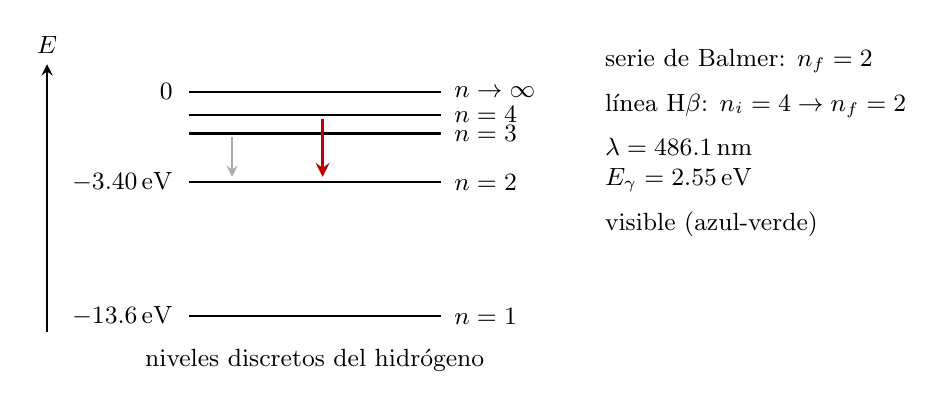
\begin{tikzpicture}[>=stealth, every node/.style={font=\small}]
        \draw[->,thick] (0,0.15) -- (0,3.55) node[above] {$E$};
        \draw[thick] (1.8,0.35) -- (5.0,0.35);
        \draw[thick] (1.8,2.05) -- (5.0,2.05);
        \draw[thick] (1.8,2.67) -- (5.0,2.67);
        \draw[thick] (1.8,2.91) -- (5.0,2.91);
        \draw[thick] (1.8,3.2) -- (5.0,3.2);
        \node[left,align=right] at (1.72,0.35) {$-13.6\,\mathrm{eV}$};
        \node[left,align=right] at (1.72,2.05) {$-3.40\,\mathrm{eV}$};
        \node[left,align=right] at (1.72,3.2) {$0$};
        \node[right] at (5.05,0.35) {$n=1$};
        \node[right] at (5.05,2.05) {$n=2$};
        \node[right] at (5.05,2.67) {$n=3$};
        \node[right] at (5.05,2.91) {$n=4$};
        \node[right] at (5.05,3.2) {$n\to\infty$};

        \draw[->,very thick,red!75!black] (3.5,2.86) -- (3.5,2.12);
        \draw[->,thick,gray!65] (2.35,2.63) -- (2.35,2.12);
        \node[align=left] at (9.0,2.55)
            {serie de Balmer: $n_f=2$\\[5pt]
             línea H$\beta$: $n_i=4\to n_f=2$\\[5pt]
             $\lambda=486.1\,\mathrm{nm}$\\
             $E_\gamma=2.55\,\mathrm{eV}$\\[5pt]
             visible (azul-verde)};
        \node[below] at (3.4,0.05) {niveles discretos del hidrógeno};
    \end{tikzpicture}
    \caption{Niveles de energía del hidrógeno y transiciones hacia $n_f=2$. La flecha roja indica la línea H$\beta$ observada en la nebulosa.}
    \label{fig:serie-balmer}
\end{figure}

    \item Un fotón de rayos X de energía inicial $1.0 \times 10^5\,\mathrm{eV}$ que viaja en la dirección $+x$ incide sobre un electrón libre en reposo. El fotón se dispersa en ángulo recto en la dirección $+y$. Encuentre las componentes del impulso del electrón que retrocede.

    \textit{Solución.} La conservación relativista de energía y momento en la dispersión Compton da, para un ángulo $\theta$ entre los fotones incidente y dispersado,
    \[
        E'_\gamma=\frac{E_\gamma}{1+(E_\gamma/m_ec^2)(1-\cos\theta)}.
    \]
    Aquí $\theta=90^\circ$ y $m_ec^2=511\,\mathrm{keV}$, por lo que $E'_\gamma=83.6\,\mathrm{keV}$. Por conservación del momento, el impulso del electrón es la diferencia entre los impulsos de los fotones:
    \[
        p_{e,x}=\frac{E_\gamma}{c}=1.00\times10^5\,\mathrm{eV}/c,
        \qquad
        p_{e,y}=-\frac{E'_\gamma}{c}=-8.36\times10^4\,\mathrm{eV}/c.
    \]
    Así, $\vec p_e=(1.00\times10^5\,\hat{x}-8.36\times10^4\,\hat{y})\,\mathrm{eV}/c$. El signo negativo indica que el electrón retrocede en dirección $-y$. \parencite[Secs. 16.2--16.2.1, pp. 525--528]{chaparro2026}
    \begin{figure}[htbp]
    \centering
    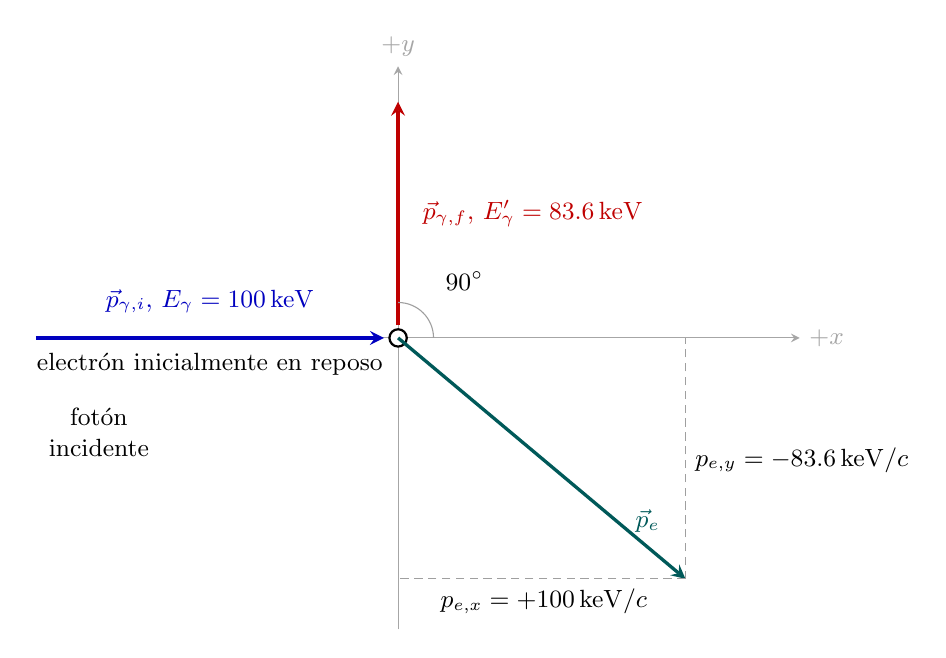
\begin{tikzpicture}[>=stealth, every node/.style={font=\small}]
        \draw[->,gray!70] (-0.45,0) -- (5.1,0) node[right] {$+x$};
        \draw[->,gray!70] (0,-3.7) -- (0,3.45) node[above] {$+y$};
        \filldraw[fill=white,draw=black,thick] (0,0) circle (0.11);
        \node[below left=2pt] at (0,0) {electrón inicialmente en reposo};

        \draw[->,very thick,blue!75!black] (-4.6,0) -- (-0.18,0)
            node[midway,above=5pt] {$\vec p_{\gamma,i}$, $E_\gamma=100\,\mathrm{keV}$};
        \draw[->,very thick,red!75!black] (0,0.16) -- (0,3.0)
            node[midway,right=5pt] {$\vec p_{\gamma,f}$, $E'_\gamma=83.6\,\mathrm{keV}$};
        \draw[->,very thick,teal!70!black] (0,0) -- (3.65,-3.06)
            node[pos=0.76,right=3pt] {$\vec p_e$};
        \draw[densely dashed,gray!75] (3.65,-3.06) -- (3.65,0);
        \draw[densely dashed,gray!75] (3.65,-3.06) -- (0,-3.06);
        \node[below] at (1.85,-3.06) {$p_{e,x}=+100\,\mathrm{keV}/c$};
        \node[right] at (3.65,-1.55) {$p_{e,y}=-83.6\,\mathrm{keV}/c$};
        \draw[gray!75] (0.45,0) arc[start angle=0,end angle=90,radius=0.45];
        \node[above right] at (0.48,0.48) {$90^\circ$};
        \node[align=center] at (-3.8,-1.2) {fotón\\incidente};
    \end{tikzpicture}
    \caption{Geometría de la dispersión Compton a $90^\circ$. La conservación vectorial del momento, $\vec p_e=\vec p_{\gamma,i}-\vec p_{\gamma,f}$, fija el retroceso del electrón y sus componentes.}
    \label{fig:compton-recoil}
\end{figure}

    \item En el efecto Sunyaev--Zel'dovich térmico (efecto Compton inverso), un cúmulo de galaxias rico contiene un medio intracumular (ICM) de gas totalmente ionizado y caliente con el que interactúan fotones del fondo cósmico de microondas (CMB). Suponga que la población de electrones tiene una temperatura $T_e = 8\,\mathrm{keV}$ y una densidad uniforme $n_e = 3.0 \times 10^{-3}\,\mathrm{cm}^{-3}$ a lo largo de un camino $L = 1.0\,\mathrm{Mpc}$ que atraviesa el centro del cúmulo. Considere que cada fotón gana una energía
    \[
        \left\langle \frac{\Delta E}{E} \right\rangle = \frac{k_B T_e}{m_e c^2}
    \]
    luego de cada colisión con un electrón.
    \begin{enumerate}
        \item[(a)] Demuestre que el parámetro Compton térmico que cuantifica la ganancia total a lo largo de la línea de visión
        \[
            y = \frac{\Delta E}{E} = \left\langle \frac{\Delta E}{E} \right\rangle \times P(\text{colisión})
        \]
        viene dado por
        \[
            y = \frac{k_B T_e}{m_e c^2}\,\sigma_T \int n_e\,d\ell,
        \]
        y calcule su valor para el cúmulo. (Aquí $\sigma_T = 6.65 \times 10^{-29}\,\mathrm{m}^2$ es la sección eficaz de interacción electrón-fotón (dispersión Thomson).)

        \textit{Solución.} La probabilidad de dispersión a lo largo de la trayectoria está determinada por la profundidad óptica $\tau=\sigma_T\int n_e\,d\ell$. Como $\tau\ll1$, la probabilidad de una colisión es $P(\text{colisión})\simeq\tau$. Al multiplicarla por la ganancia media por colisión dada en el enunciado,
        \[
            y=\left\langle\frac{\Delta E}{E}\right\rangle P(\text{colisión})
            =\frac{k_BT_e}{m_ec^2}\,\sigma_T\int n_e\,d\ell.
        \]
        Para los valores del cúmulo, $k_BT_e/(m_ec^2)=8/511=1.57\times10^{-2}$, $n_e=3.0\times10^3\,\mathrm{m}^{-3}$ y $L=3.086\times10^{22}\,\mathrm{m}$. Entonces
        \[
            \tau=\sigma_T n_eL=6.16\times10^{-3},
            \qquad y=(1.57\times10^{-2})(6.16\times10^{-3})
            =9.64\times10^{-5}.
        \]
        \parencite[Sec. 16.2.2, pp. 532--533]{chaparro2026}

        \item[(b)] En longitudes de onda milimétricas, la dependencia completa en frecuencia de la variación de la intensidad relativa se aproxima por la función
        \[
            \frac{\Delta I(\nu)}{I_0(\nu)} = y\left[x\coth\left(\frac{x}{2}\right)-4\right],
            \qquad
            x = \frac{h\nu}{k_B T_{\mathrm{CMB}}}.
        \]
        Evalúe la variación fraccionaria de intensidad $\Delta I/I_0$ en $\nu = 150\,\mathrm{GHz}$ e indique si la señal del CMB se observa en emisión o en absorción a dicha frecuencia.

        \textit{Solución.} Tomamos $T_{\mathrm{CMB}}=2.725\,\mathrm{K}$. Entonces,
        \[
            x=\frac{h\nu}{k_BT_{\mathrm{CMB}}}=2.642,
            \qquad x\coth(x/2)-4=-0.953.
        \]
        Con el valor de $y$ obtenido en (a),
        \[
            \frac{\Delta I}{I_0}=y[-0.953]=-9.18\times10^{-5}.
        \]
        El signo negativo indica una disminución de intensidad: a $150\,\mathrm{GHz}$ se observa un decremento o absorción del CMB por el efecto SZ térmico. \parencite[Sec. 16.2.2, pp. 532--533]{chaparro2026}
        \begin{figure}[htbp]
    \centering
    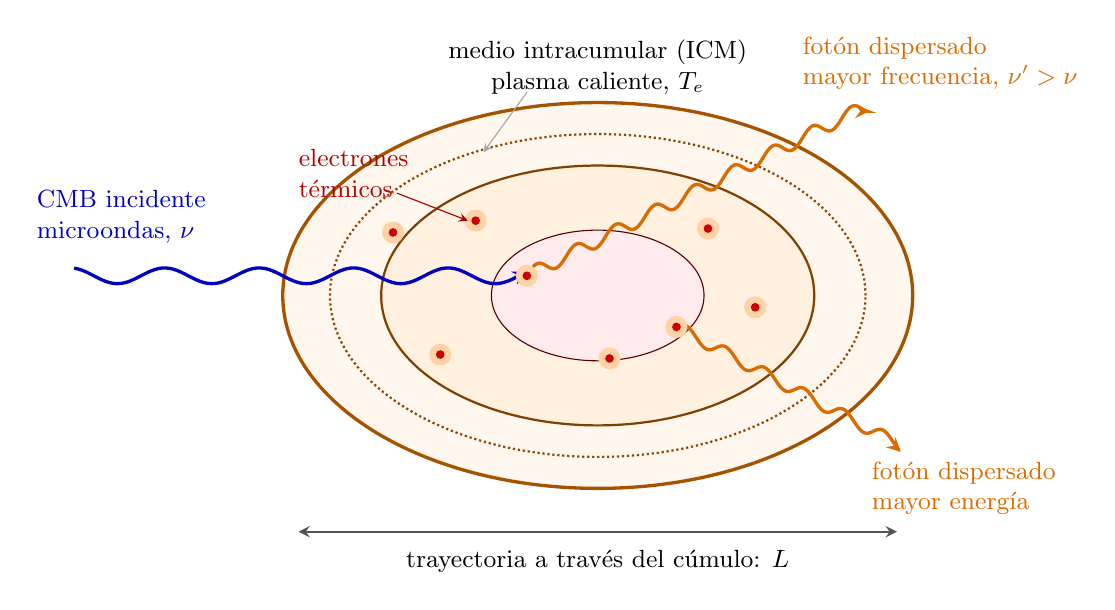
\begin{tikzpicture}[>=stealth, every node/.style={font=\small}]
        \draw[fill=orange!7,draw=orange!65!black,very thick] (7,0) ellipse (4.0cm and 2.45cm);
        \draw[fill=orange!12,draw=orange!50!black,thick] (7,0) ellipse (2.75cm and 1.65cm);
        \draw[fill=red!8,draw=red!35!black] (7,0) ellipse (1.35cm and 0.83cm);
        \draw[orange!55!black,densely dotted,thick] (7,0) ellipse (3.4cm and 2.05cm);

        \node[align=center] at (7,2.9) {medio intracumular (ICM)\\plasma caliente, $T_e$};
        \draw[->,gray!70,thin] (6.1,2.58) -- (5.55,1.82);

        \draw[->,very thick,blue!75!black,domain=0.35:6.1,samples=120,smooth]
            plot (\x,{0.25+0.10*sin(300*\x)});
        \draw[->,very thick,orange!85!black,domain=6.1:10.45,samples=140,smooth]
            plot (\x,{0.25+0.50*(\x-6.1)+0.09*sin(720*(\x-6.1))});
        \draw[->,very thick,orange!85!black,domain=8.0:10.85,samples=120,smooth]
            plot (\x,{-0.4-0.53*(\x-8.0)+0.08*sin(720*(\x-8.0))});

        \foreach \x/\y in {4.4/0.8,5.0/-0.75,5.45/0.95,6.1/0.25,7.15/-0.8,8.0/-0.4,8.4/0.85,9.0/-0.15}
        {
            \fill[orange!35] (\x,\y) circle (0.14);
            \fill[red!80!black] (\x,\y) circle (0.055);
        }
        \node[red!70!black,align=left] at (3.9,1.55) {electrones\\térmicos};
        \draw[->,red!65!black] (4.45,1.3) -- (5.35,0.95);

        \node[blue!75!black,align=left] at (0.95,1.0) {CMB incidente\\microondas, $\nu$};
        \node[orange!85!black,align=left] at (11.35,2.95)
            {fotón dispersado\\mayor frecuencia, $\nu'>\nu$};
        \node[orange!85!black,align=left] at (11.65,-2.45)
            {fotón dispersado\\mayor energía};

        \draw[<->,gray!65!black,thick] (3.2,-3.0) -- (10.8,-3.0)
            node[midway,below=3pt,text=black] {trayectoria a través del cúmulo: $L$};
    \end{tikzpicture}
    \caption{Esquema del efecto Sunyaev--Zel'dovich térmico: los fotones de baja energía del CMB atraviesan el ICM y, al dispersarse con electrones calientes, ganan energía. La intensidad del efecto depende del parámetro $y=(k_BT_e/m_ec^2)\,\sigma_T\int n_e\,d\ell$.}
    \label{fig:efecto-sz}
\end{figure}
    \end{enumerate}

    \item Para un átomo de H ¿Cuál es la probabilidad de encontrar al electrón entre $r = 0$ y $r = a_0$ para el nivel $n = 2$ comparando los niveles $l = 0$ y $l = 1$?

    \textit{Solución.} La probabilidad radial entre $r_1$ y $r_2$ es $\int_{r_1}^{r_2}r^2|R_{n\ell}(r)|^2\,dr$. Para $n=2$, las funciones radiales normalizadas son
    \[
        R_{20}(r)=\frac{1}{2\sqrt{2}\,a_0^{3/2}}\left(2-\frac{r}{a_0}\right)e^{-r/(2a_0)},
        \qquad
        R_{21}(r)=\frac{1}{2\sqrt{6}\,a_0^{3/2}}\frac{r}{a_0}e^{-r/(2a_0)}.
    \]
    Con $u=r/a_0$, para los dos estados se obtiene
    \[
        P_{2s}(0\leq r\leq a_0)=\frac18\int_0^1u^2(2-u)^2e^{-u}\,du
        =1-\frac{21}{8e}\simeq0.0343,
    \]
    \[
        P_{2p}(0\leq r\leq a_0)=\frac1{24}\int_0^1u^4e^{-u}\,du
        =1-\frac{65}{24e}\simeq0.00366.
    \]
    Por tanto, dentro de $a_0$ la probabilidad para $\ell=0$ es aproximadamente $9.38$ veces la de $\ell=1$. \parencite[Sec. 20.4, pp. 675--676; Sec. 20.5, pp. 679--680]{chaparro2026}
    \begin{figure}[htbp]
    \centering
    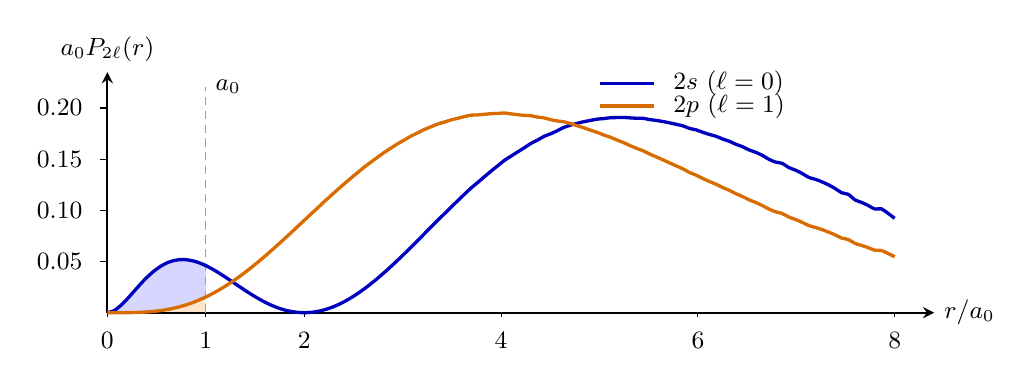
\begin{tikzpicture}[>=stealth, every node/.style={font=\small},x=1.25cm,y=13cm]
        \fill[blue!16]
            plot[domain=0:1,samples=30] (\x,{\x*\x*(2-\x)*(2-\x)*exp(-\x)/8})
            -- (1,0) -- (0,0) -- cycle;
        \fill[orange!20]
            plot[domain=0:1,samples=30] (\x,{\x*\x*\x*\x*exp(-\x)/24})
            -- (1,0) -- (0,0) -- cycle;
        \draw[->,thick] (0,0) -- (8.4,0) node[right] {$r/a_0$};
        \draw[->,thick] (0,0) -- (0,0.235) node[above] {$a_0P_{2\ell}(r)$};
        \foreach \x in {0,1,2,4,6,8}
            \draw (\x,0) -- (\x,-0.004) node[below=2pt] {\x};
        \foreach \y/\lab in {0.05/0.05,0.10/0.10,0.15/0.15,0.20/0.20}
            \draw (0,\y) -- (-0.07,\y) node[left=3pt] {\lab};
        \draw[densely dashed,gray!75] (1,0) -- (1,0.22);
        \node[above right] at (1,0.205) {$a_0$};
        \draw[very thick,blue!75!black,domain=0:8,samples=120,smooth]
            plot (\x,{\x*\x*(2-\x)*(2-\x)*exp(-\x)/8});
        \draw[very thick,orange!85!black,domain=0:8,samples=120,smooth]
            plot (\x,{\x*\x*\x*\x*exp(-\x)/24});
        \draw[blue!75!black,very thick] (5.0,0.224) -- (5.55,0.224);
        \node[anchor=west] at (5.65,0.224) {$2s\ (\ell=0)$};
        \draw[orange!85!black,very thick] (5.0,0.202) -- (5.55,0.202);
        \node[anchor=west] at (5.65,0.202) {$2p\ (\ell=1)$};
    \end{tikzpicture}
    \caption{Densidades radiales $P_{2\ell}(r)=r^2|R_{2\ell}(r)|^2$ en unidades adimensionales. El área sombreada entre el origen y $a_0$ representa las probabilidades $P_{2s}\simeq0.0343$ y $P_{2p}\simeq0.00366$; el estado $2s$ es unas $9.38$ veces más probable en esa región.}
    \label{fig:probabilidad-radial}
\end{figure}

    \item Asumiendo un modelo hidrogenoide, calcule la longitud de onda de la transición fundamental $n = 2 \to 1$ para el Fe e identifique el rango del espectro electromagnético correspondiente.
    \[
        A_{21} = 6.3 \times 10^8\,\mathrm{s}^{-1}.
    \]
    \textit{Solución.} Para un ion hidrogenoide, $1/\lambda=R_\infty Z^2(1/n_f^2-1/n_i^2)$. Tomamos $Z=26$ para el hierro y $n_i=2$, $n_f=1$:
    \[
        \frac{1}{\lambda}= (1.097\times10^7\,\mathrm{m}^{-1})(26)^2\left(1-\frac14\right)
        =5.56\times10^9\,\mathrm{m}^{-1},
        \qquad \lambda=1.80\times10^{-10}\,\mathrm{m}=0.180\,\mathrm{nm}.
    \]
    Corresponde a un fotón de rayos X. El coeficiente $A_{21}$ no interviene en el cálculo de la longitud de onda; describe la probabilidad de transición espontánea por unidad de tiempo. \parencite[Sec. 15.5, p. 496; Sec. 20.4, pp. 675--676]{chaparro2026}
    \begin{figure}[htbp]
    \centering
    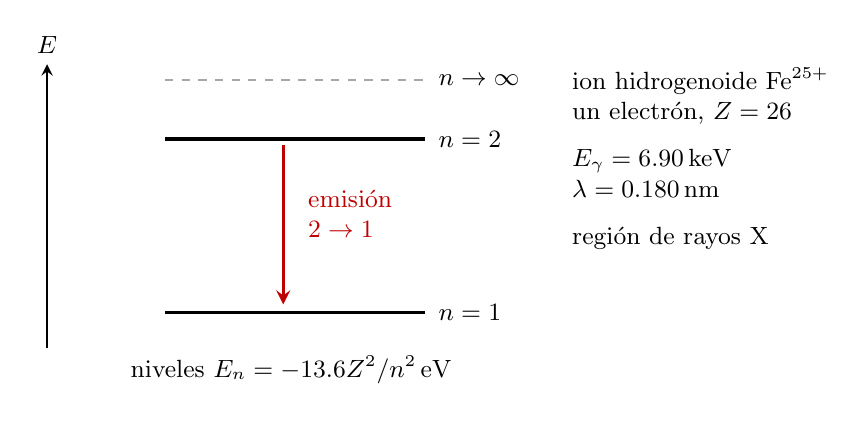
\begin{tikzpicture}[>=stealth, every node/.style={font=\small}]
        \draw[->,thick] (0,0.1) -- (0,3.7) node[above] {$E$};
        \draw[very thick] (1.5,0.55) -- (4.8,0.55);
        \draw[very thick] (1.5,2.75) -- (4.8,2.75);
        \draw[thick,dashed,gray!70] (1.5,3.5) -- (4.8,3.5);
        \node[right] at (4.85,0.55) {$n=1$};
        \node[right] at (4.85,2.75) {$n=2$};
        \node[right] at (4.85,3.5) {$n\to\infty$};
        \draw[->,very thick,red!75!black] (3.0,2.68) -- (3.0,0.65);
        \node[red!75!black,align=left] at (3.85,1.8) {emisión\\$2\to1$};
        \node[align=left] at (8.3,2.5)
            {ion hidrogenoide Fe$^{25+}$\\un electrón, $Z=26$\\[6pt]
             $E_\gamma=6.90\,\mathrm{keV}$\\
             $\lambda=0.180\,\mathrm{nm}$\\[6pt]
             región de rayos X};
        \node[below] at (3.1,0.12) {niveles $E_n=-13.6Z^2/n^2\,\mathrm{eV}$};
    \end{tikzpicture}
    \caption{Transición $n=2\to1$ del ion de hierro hidrogenoide. La diferencia de energías determina la longitud de onda; el coeficiente de Einstein $A_{21}$ determina la tasa de transición.}
    \label{fig:fe-hidrogenoide}
\end{figure}
\end{enumerate}

\printbibliography[title={Referencias}]

\end{document}